\chapter{Introduction}
Epic introduction goes here.\\

Then you can do things like say as shown in Fig.\ \ref{fig:sample}
or add citiations to epic papers like \cite{eliassen1951}. If we also decide
to add a table, we can add a reference to Table \ref{tab:lorenz}.

\begin{table}[t]
\caption[This caption appears in the LoT]{This is a sample table caption and
  table layout from the AMS LaTeX template file.Table from Lorenz (1963).}
\label{tab:lorenz}
\begin{center}
\begin{tabular}{ccccrrcrc}
\hline\hline
$N$ & $X$ & $Y$ & $Z$\\
\hline
 0000 & 0000 & 0010 & 0000 \\
 0005 & 0004 & 0012 & 0000 \\
 0010 & 0009 & 0020 & 0000 \\
 0015 & 0016 & 0036 & 0002 \\
 0020 & 0030 & 0066 & 0007 \\
 0025 & 0054 & 0115 & 0024 \\
\hline
\end{tabular}
\end{center}
\end{table}

\begin{figure}[H]
    \centering
    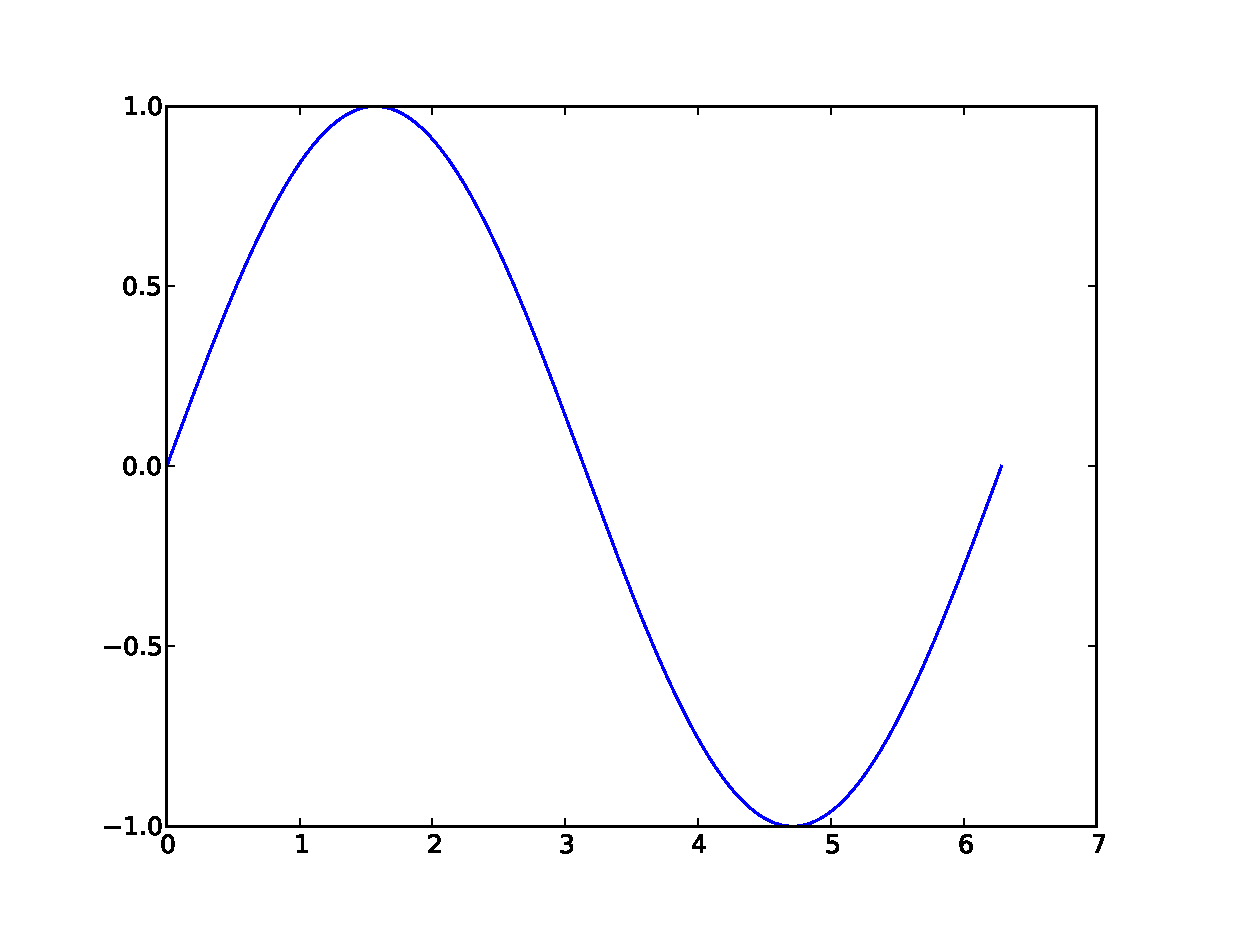
\includegraphics[width=0.75\textwidth]{./chap1/fig/sample_fig}
    \caption[This caption is only in the LoF]{This is a sample figure with a
    sample caption.}
    \label{fig:sample}
\end{figure}
